\documentclass[11pt]{article}
\usepackage{enumitem}
\usepackage{float}
\usepackage[margin=1in]{geometry}
\usepackage{graphicx}
\usepackage[space]{grffile}
\usepackage{adjustbox}
\usepackage{amsmath}
\usepackage{amsthm}
\usepackage{amssymb}
\usepackage{fullpage}
\usepackage{fancyhdr}
\usepackage{xparse}
\usepackage[makeroom]{cancel}
\newcommand{\cnum}{CM146}
\newcommand{\ced}{Fall 2018}
\newcommand{\ctitle}[3]{\title{\vspace{-0.5in}\cnum, \ced\\Problem Set #1: #2}}
\newcommand{\solution}[1]{{{\color{blue}{\bf Solution:} {#1}}}}
\NewDocumentCommand{\texcod}{mm}{%
	\texttt{\textcolor{#1}{#2}}%
}
\usepackage[usenames,dvipsnames,svgnames,table,hyperref]{xcolor}
\usepackage{listings}
\usepackage{color} %red, green, blue, yellow, cyan, magenta, black, white
\definecolor{mygreen}{RGB}{28,172,0} % color values Red, Green, Blue
\definecolor{mylilas}{RGB}{170,55,241}

\renewcommand*{\theenumi}{\alph{enumi}}
\renewcommand*\labelenumi{(\theenumi)}
\renewcommand*{\theenumii}{\roman{enumii}}
\renewcommand*\labelenumii{\theenumii.}

\author{Zheng Wang (404855295)}
\date{\today}
\title{MATH 151B Homework 3}

\begin{document}
	
\lstset{language=Matlab,%
	basicstyle=\footnotesize,
	breaklines=true,%
	morekeywords={matlab2tikz},
	keywordstyle=\color{blue},%
	morekeywords=[2]{1}, keywordstyle=[2]{\color{black}},
	identifierstyle=\color{black},%
	stringstyle=\color{mylilas},
	commentstyle=\color{mygreen},%
	showstringspaces=false,%without this there will be a symbol in the places where there is a space
	numbers=left,%
	numberstyle={\tiny \color{black}},% size of the numbers
	numbersep=9pt, % this defines how far the numbers are from the text
	emph=[1]{for,end,break},emphstyle=[1]\color{red}, %some words to emphasise
	%emph=[2]{word1,word2}, emphstyle=[2]{style},    
}

\maketitle
\section*{Question 1}
\begin{itemize}
	\item [(a)]
	The Euler's Method gives
	\[ \begin{cases}
	w_{i+1} = w_i + h\cdot f(x_i, w_i)\\
	w_0 = 0
	\end{cases} \]
	Since $ x_i = ih $, we then break down the original formula to 
	\[ \begin{cases}
	w_{i+1} = w_i + h(ih - (ih)^2)\\
	w_0 = 0
	\end{cases} \]
	\begin{align*}
	\intertext{Therefore, we have }
	w_{i+1} &= w_i + h\cdot (ih - (ih)^2 )\\
	&= w_{i-1} + h\cdot ((i-1)h - (i-1)^2 h^2) + h\cdot (ih - (ih)^2)\\
	&= w_{i-1} + (i-1)\cdot h^2 - (i-1)^2\cdot h^3 + i \cdot h^2 - i^2\cdot h^3\\
	&= w_{i-1} + h^2 \cdot [i + (i-1)] - h^3\cdot [i^2 + (i-1)^2] \\
	&= w_0 + h^2\cdot \left(\sum_{j=0}^{i}j\right) - h^3\cdot \left(\sum_{j=0}^{i}j^2\right) && (\text{By telescoping})\\
	&= h^2 \cdot \frac{i\cdot (i+1)}{2} - h^3\cdot \frac{i(i+1)(2i+1)}{6} 
	\end{align*} 
	Therefore, $ \displaystyle \boxed{w_i = h^2\cdot \frac{i(i-1)}{2} - h^3\cdot \frac{i(i-1)(2i-1)}{6} }$\hfill $ \blacksquare $\pagebreak
	
	\item [(b)]
	We take $ x = ih $, where $ x $ is an arbitary fixed point
	\begin{align*}
	\intertext{Then we have the following: }
	\lim_{h\rightarrow 0} \left|w_i - y(x)\right| &= \lim_{h\rightarrow 0} \left|\frac{i(i-1)}{2}\cdot h^2 - \frac{i(i-1)(2i-1)}{6}\cdot h^3 - \frac{i^2}{2}\cdot h^2 + \frac{i^3}{3}\cdot h^3\right| \\
	&= \lim_{h\rightarrow 0} \left|\frac{ \cancel{i^2} - i - \cancel{i^2}}{2}\cdot h^2 + \frac{-\cancel{2i^3}+3i^2-i+\cancel{2i^3}}{6}\cdot h^3\right|\\
	&= \lim_{h\rightarrow 0} \left| \frac{-ih}{2}\cdot h + \frac{(ih)^2}{2}\cdot h - \frac{ih}{6}\cdot h^2 \right|\\
	&= \lim_{h\rightarrow 0} \left| -\frac{x}{2}\cdot h + \frac{x^2}{2}\cdot h - \frac{x}{6}\cdot h^2 \right|\\
	& = \left| \lim_{h\rightarrow 0} \left( -\frac{x}{2}\cdot h + \frac{x^2}{2}\cdot h - \frac{x}{6}\cdot h^2 \right) \right|&& &\text{(By continuity)}&\\
	& = 0 && &\text{(Since $ x $ is a constant)}&
	\end{align*}
	Thus, Euler's method is convergent. \hfill $ \blacksquare $
\end{itemize}

\section*{Question 2}
The RKF12 method is implemented with the following code.
\lstinputlisting{Run_rkf12.m}\hfill\\
\textbf{Explanation:}
\begin{align*}
\intertext{From formula of Modified Euler Method and Euler Method, we have the following:}
&& &\tilde{w}_{i+1} = w_i + \frac{h}{2}\left[f(t_i,w_i) + f(t_i + h , w_i + hf(t_i,w_i)) \right]&\\
&& &w_{i+1} = w_i + h\cdot f(t_i,w_i)&\\
\intertext{Then, we compute $ \tau_{i+1} $ and $ \tilde{\tau}_{i+1} $:}
&& \tau_{i+1} &= \frac{y(t_{i+1})-w_i}{h} - f(t_i,w_i)&\\
&& &=\frac{y(t_{i+1})-(w_i+hf(t_i,w_i))}{h} = \frac{1}{h}\left(y(t_{i+1})-w_{i+1}\right)&\\
&& \tilde{\tau}_{i+1} &= \frac{y(t_{i+1})-(w_i + \frac{h}{2}\left[f(t_i,w_i) + f(t_i + h , w_i + hf(t_i,w_i)) \right] )}{h}&\\
&& &=\frac{1}{h}\left(y(t_{i+1})-\tilde{w}_{i+1}\right)&\\
\end{align*}
\begin{align*}
\intertext{Next, we arrive at the following:}
&& \tau_{i+1} &= \frac{1}{h}\left(y(t_{i+1})-w_{i+1}\right) = \frac{1}{h}\left[\left(y(t_{i+1})-\tilde{w}_{i+1}\right) + \left(\tilde{w}_{i+1} - w_{i+1}\right)\right]&\\
&& &= \tilde{\tau}_{i+1} + \frac{1}{h}(\tilde{w}_{i+1}-w_{i+1})&
\intertext{As $ \tilde{\tau}_{i+1} $ is $\mathcal{O}(h^2)$, but $ \tau_{i+1} $ is $ \mathcal{O}(h) $. Thus, $ \frac{1}{h}(\tilde{w}_{i+1}-w_{i+1}) $ is $ \mathcal{O}(h) $. Therefore, $\tau_{i+1} \approx \frac{1}{h}(\tilde{w}_{i+1}-w_{i+1}) $. With this equation, we can estimate the local truncation error as: }
&& &R = \frac{1}{h}\left|\tilde{w}_{i+1}-w_{i+1} \right| \approx \tau_{i+1} &
\end{align*}

In our program, since we have $ \tilde{w}_{i+1} = w_i + K3 $ and $ w_{i+1} = w_i + K1 $, Therefore, we have $ R = \frac{1}{h}\left|K3 - K1\right| $. Finally, by taking $ \tau_{i+1}(h) \approx Kh $, by solving $ \tau_{i+1}(qh) \approx Kqh \approx q\tau_{i+1}(h) \approx qR \le \epsilon $, we get $ q \le \frac{\epsilon}{R} $. To be more conservative, we make $ q $ even smaller by let $ q = \frac{\epsilon}{2R} $. Since in the program $ TOL $ represent $ \epsilon $, we use $ q = TOL/2R $ in the program.

After these, to make sure the $ q $ is not too small nor too large , we also bound $ q $ with $ 0.1 $ and $ 4 $. To make sure that $ h $ is reasonable, we also fix $\text{hmin} \le  h \le \text{hmax} $ in the program. From the demo I did in the program, the final estimation is $ 2.7181 $, which is close to the real solution $ 2.7183 $ to degree $ 10^{-4} $.\\\\

In terms of the run-time of the RKF12 and RKF45 method, when the accuracy is low (like $ 10^{-2} $), the two method will have similar performance, sometimes RKF12 can run faster than RKF45. This is because we have fixed the maximum step size in the program, and even though RKF45 can achieve the desired accuracy level with large step size, the program with still have to run the a minimum number of steps. Moreover, since RKF45 must take more calculations per iteration than RKF12, it might have very similar or even lower performance than RKF12.

But when accuracy is fixed high (like $ 10^{-7} $), the RKF45 can run much faster than RKF12. This is becuase to achieve the desired accuracy level, RKF12 will need to take much smaller step size than RKF45. Even though RKF45 needs more evaluation per iteration, there are much less iterations to run. Therefore, it is much faster than RKF12. The general trend in the performance is given by the following plot:\\
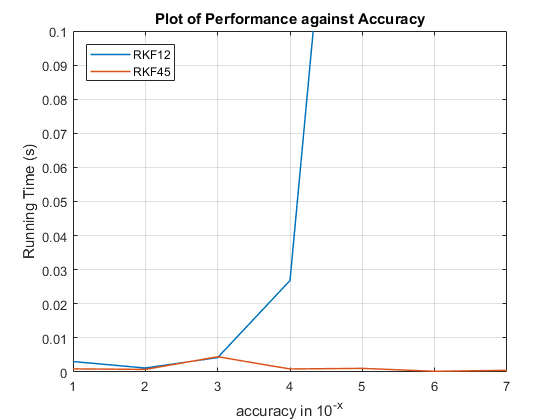
\includegraphics{performance.png}\\\\
The following code is used to do the test:\\
\lstinputlisting{compare.m}



\end{document}